% !TeX spellcheck = id_ID
\documentclass[a4paper,12pt]{article}
\usepackage[bahasa]{babel}
\usepackage{graphicx}
\usepackage{multirow}
\usepackage{enumitem}
\usepackage{listings}
\usepackage{wrapfig}
\usepackage[T1]{fontenc}
\usepackage{inconsolata}

\usepackage{color}
\usepackage[table]{xcolor}
\definecolor{pblue}{rgb}{0.13,0.13,1}
\definecolor{pgreen}{rgb}{0,0.5,0}
\definecolor{pred}{rgb}{0.9,0,0}
\definecolor{pgrey}{rgb}{0.46,0.45,0.48}
\lstset{language=Java,
	showspaces=false,
	showtabs=false,
	breaklines=true,
	showstringspaces=false,
	breakatwhitespace=true,
	commentstyle=\color{pgreen},
	keywordstyle=\color{pblue},
	stringstyle=\color{pred},
	basicstyle=\ttfamily,
	moredelim=[il][\textcolor{pgrey}]{$$},
	moredelim=[is][\textcolor{pgrey}]{\%\%}{\%\%}
}

\graphicspath{ {./img/} }
\begin{document}
\title{ {\Large Laporan Praktikum}\\ Algoritma dan Pemrograman \\{\Large Pertemuan 7}}

\author{Aldzikri Dwijayanto Prathama 
	\\195410189
	\\Teknik Informatika}
\makeatletter
\begin{titlepage}
	\begin{center}
		{\huge \bfseries \@title }\\[14ex]
		
\includegraphics[scale=.8]{logo}\\[4ex]
		{\large \@author}\\[19ex]
		{\large \bfseries {SEKOLAH TINGGI MANAJEMEN INFORMATIKA DAN KOMPUTER
				AKAKOM YOGYAKARTA}}
	\end{center}


%{\large \@date} 
\end{titlepage}
\makeatother
%\maketitle
\newpage
\tableofcontents
\newpage

\section{Tujuan}
Mahasiswa dapat mengimplementasikan konsep seleksi bertingkat untuk menyelesaikan kasus 
\section{Dasar Teori}
\paragraph{}
Seleksi pernah dipelajar pada pertemuan modul 5 dan 6 baik menggunakan if maupun
switch-case. Seleksi bertingkat dapat diartikan sebagai seleksi di dalam seleksi. Beberapa bentuk kemungkinan seleksi bertingkat dua dapat dilihat seperti di bawah :
\begin{table}[!ht]
	\begin{tabular}{|l|l|l|}
		\hline
		\rowcolor[HTML]{E5B9B7}
		\multicolumn{1}{|c|}{\cellcolor[HTML]{E5B9B7} Bentuk 1} & \multicolumn{1}{c|}{\cellcolor[HTML]{E5B9B7} Bentuk 2} & \multicolumn{1}{c|}{\cellcolor[HTML]{E5B9B7} Bentuk 3} \\ \hline
		
		{\begin{lstlisting}
if(kondisi1)
{
  Pernyataan1;
}
else
{
if(kondisi2)
  Pernyataan2;
else
  Pernyataan3;
}
			
		\end{lstlisting}}&
{\begin{lstlisting}[language=Java]
if(kondisi1)
{
  if(kondisi2)
    Pernyataan1;
  else
    Pernyataan2;
}
else
{
  Pernyataan3;
}
	\end{lstlisting}}
	
	                               &
{\begin{lstlisting}[language=Java]
if(kondisi1)
{
  if(kondisi2)
    Pernyataan1;
  else
    Pernyataan2;
}
else
{
  if(kondisi3)
    Pernyataan3;
  else
    Pernyataan4;
}
\end{lstlisting}}
	                                                              \\ \hline
	\end{tabular}
\end{table}\\
Keterangan:
\paragraph{Bentuk 1}
\begin{itemize}
	\item Jika kondisi 1 bernilai Benar, maka akan dikerjakan Pernyataan 1,
	\item Jika kondisi 1 bernilai Salah, maka akan mengerjakan bagian else. Bagian else
	akan dikerjakan dimulai dengan pengecekan kondisi 2, jika kondisi 2 bernilai
	Benar, maka Pernyataan 2 akan dikerjakan, jika kondisi 2 bernilai Salah, maka
	Pernyataan 3 yang akan dikerjakan.
\end{itemize}
\paragraph{Bentuk 2}
\begin{itemize}
	\item Jika kondisi 1 bernilai Benar, maka akan dikerjakan statement yang ada didalam
	if yaitu dimulai dari pengecekan kondisi 2, jika kondisi 2 bernilai Benar, maka
	Pernyataan 1 akan dikerjakan, tetapi jika kondisi 2 bernilai Salah, maka
	Pernyataan 2 yang akan dikerjakan.
	\item Jika kondisi 1 bernilai Salah, maka Pernyataan 3 yang akan dikerjakan.
\end{itemize}
\paragraph{Bentuk 3}
\begin{itemize}
	\item Jika kondisi 1 bernilai Benar, maka akan dikerjakan statement yang ada didalam
	if yaitu dimulai dari pengecekan kondisi 2, jika kondisi 2 bernilai Benar, maka
	Pernyataan 1 akan dikerjakan, tetapi jika kondisi 2 bernilai Salah, maka
	Pernyataan 2 yang akan dikerjakan.
	\item Jika kondisi 1 bernilai Salah, maka akan mengerjakan bagian else. Bagian else
	akan dikerjakan dimulai dengan pengecekan kondisi 3, jika kondisi 3 bernilai
	Benar, maka Pernyataan 3 akan dikerjakan, tetapi jika kondisi 3 bernilai Salah,
	maka Pernyataan 4 yang akan dikerjakan.
\end{itemize}
\paragraph{Flowchart Bentuk 1\\}
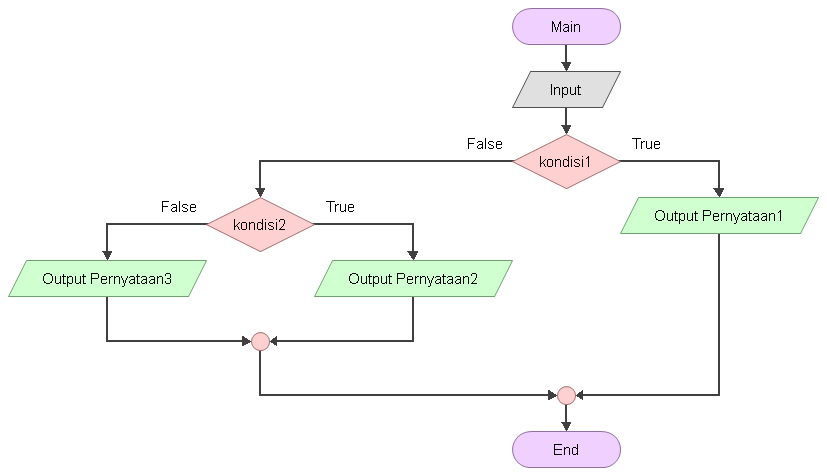
\includegraphics[width=\linewidth]{modimage--011}
\paragraph{Flowchart Bentuk 2\\}
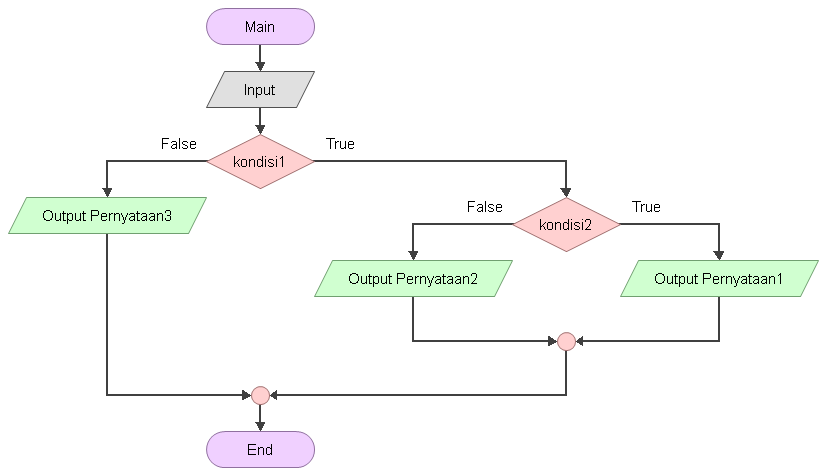
\includegraphics[width=\linewidth]{modimage--012}
\paragraph{Flowchart Bentuk 3\\}
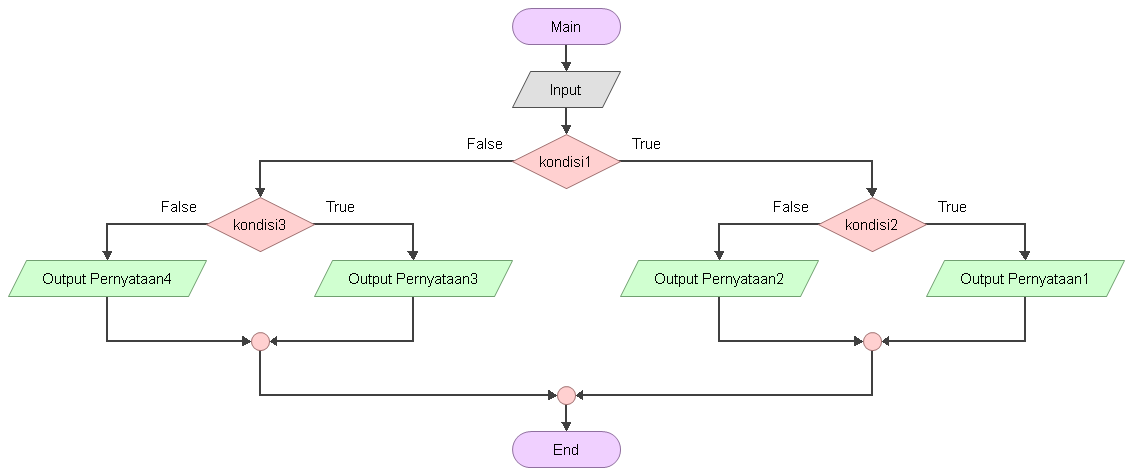
\includegraphics[width=\linewidth]{modimage--013}
\paragraph{}
Selain bentuk 1, bentuk 2, dan bentuk 3, masih ada bentuk-bentuk seleksi bertingkat
yang lain, misalnya, if-else if didalam if, if di dalam switch, switch di dalam if, dan lain-
lain.
\section{Praktik}
\subsection{Praktik 1}
\paragraph{Masalah\\}
Ketik program di bawah:\\
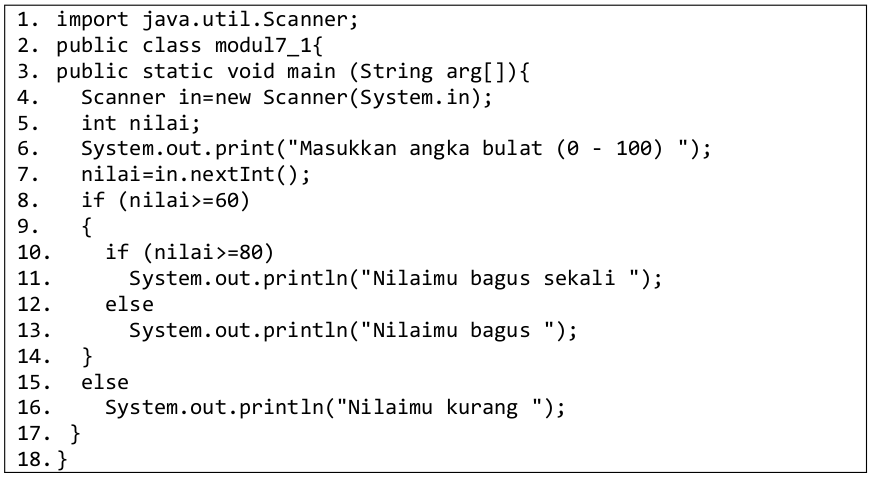
\includegraphics[width=\linewidth]{code1}\\
\begin{enumerate}[label=\alph*.]
	\item Jalankan program, masukkan nilai 70, amati hasilnya, jelaskan!
	\item Jalankan program, masukkan nilai 90, amati hasilnya, jelaskan!
	\item Jalankan program, masukkan nilai 50, amati hasilnya, jelaskan!
\end{enumerate}
\paragraph{Penyelesaian\\}
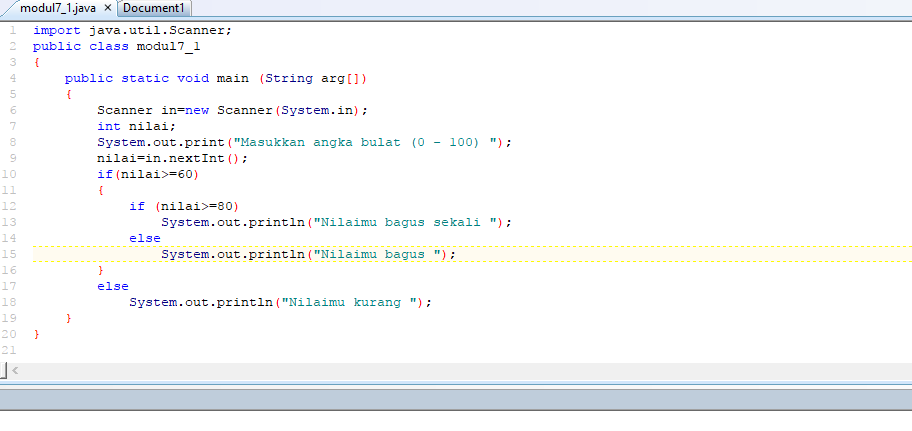
\includegraphics[width=\linewidth]{image--000}

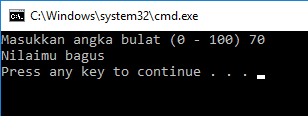
\includegraphics[scale=0.6]{image--001}

Jika program dimasukkan dengan angka 70, maka akan menghasilkan output nilaimu bagus, karena input memenuhi kondisi if pertama tetapi tidak dengan kondisi kedua, sehingga program menjalankan \texttt{System.out.println("Nilaimu bagus ");}\\

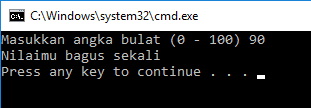
\includegraphics[scale=0.6]{image--002}

Sedangkan jika program dimasukkan dengan angka 90, maka akan menghasilkan output nilaimu bagus sekali, karena input memenuhi kondisi if pertama dan kedua, sehingga program menjalankan\\ \texttt{System.out.println("Nilaimu bagus sekali");}\\

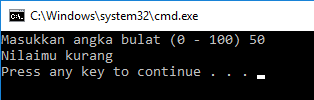
\includegraphics[scale=0.6]{image--003}

Lalu jika program dimasukkan dengan angka 50, maka akan menghasilkan output nilaimu kurang, karena input tidak memenuhi kondisi if pertama, sehingga langsung masuk ke \texttt{else}, lalu program menjalankan\\ \texttt{System.out.println("Nilaimu kurang");}

\subsection{Praktik 2}
\paragraph{Masalah\\}
Modifikasi praktik 1, dengan ketentuan :
Jika nilai < 60, maka ada proses seleksi lagi yaitu :
\begin{itemize}
	\item Jika nilai >= 30 maka akan ditampilkan nilaimu kurang
	\item Jika nilai < 30 maka akan ditampilkan nilaimu jelek
\end{itemize}
\paragraph{Penyelesaian\\}
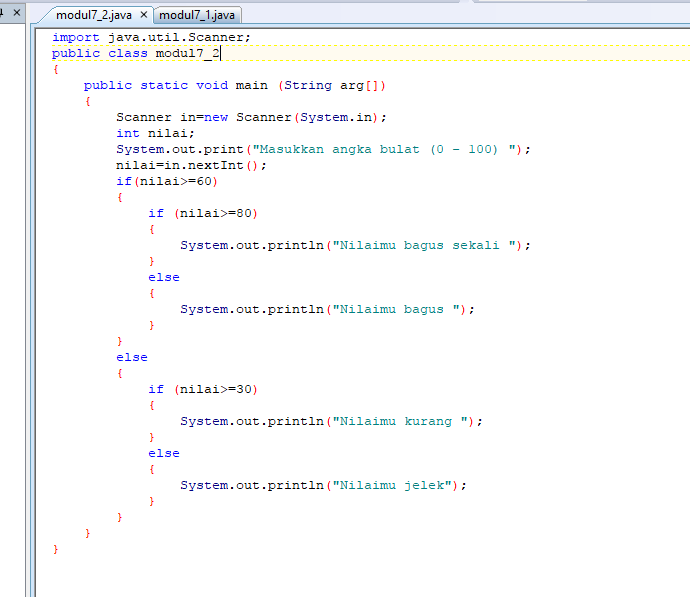
\includegraphics[width=\linewidth]{image--004}\\
Dari gambar diatas bisa terlihat, ditambahkan:
\begin{lstlisting}[language=Java]
if (nilai>=30)
{
	System.out.println("Nilaimu kurang ");
}
else
{
	System.out.println("Nilaimu jelek");
}
\end{lstlisting}
kedalam \texttt{else}, karena \texttt{if} memiliki kondisi nilai >=60, berarti <=60 akan masuk ke \texttt{else}, oleh karena itu kode di atas ditambahkan ke dalam else, untuk menyeleksi kembali nilai yang kurang dari sama dengan 60. Sehinnga jika dijalankan outputnnya menjadi\\
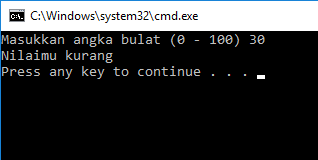
\includegraphics[scale=0.6]{image--005}
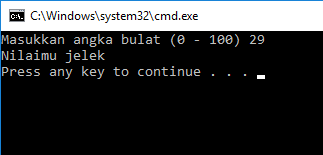
\includegraphics[scale=0.6]{image--006}
\subsection{Praktik 3}
\paragraph{Masalah\\}
Ketik program di bawah
\begin{lstlisting}
import java.util.Scanner;
public class modul7_3{
public static void main (String arg[]){
    Scanner in=new Scanner(System.in);
    Scanner masuk=new Scanner(System.in);
    String pil, jenis;
    System.out.println("Hitung persegi/lingkaran");
    System.out.println("===========================");
    System.out.print("masukkan pilihan : ");
    pil=in.next();
    switch(pil)
    {
        case "persegi":
            int sisi;
            System.out.print("masukkan sisi : ");
            sisi=masuk.nextInt();
            System.out.print("luas/keliling : ");
            jenis=in.next();
            switch(jenis)
            {
                case "luas":
                    int luas=sisi*sisi;
                    System.out.println("Luas persegi : "+luas);
                    break;
                case "keliling":
                    int kel=4*sisi;
                        System.out.println("Keliling persegi : "+kel);
                    break;
                default:
                    System.out.println("Salah masukkan jenis");
            }
            break;
            case "lingkaran":
            double jari;    
            System.out.print("masukkan jari-jari : ");
            jari=masuk.nextDouble();
            System.out.print("luas/keliling : ");
            jenis=in.next();
            switch(jenis)
            {
                case "luas":
                    double luasl=3.14*jari*jari;
                    System.out.println("Luas lingkaran : "+luasl);
                    break;
                case "keliling":
                    double kell=2*3.14*jari;
                    System.out.println("Luas lingkaran : "+kell);
                    break;
                default:
                    System.out.println("Salah masukkan jenis");
            }
            break;
            default:
            System.out.println("Salah masukkan pilihan");
        }
}
}
\end{lstlisting}
\begin{enumerate}[label=\alph*.]
	\item Jalankan program diatas dengan menguji beberapa kemungkinan pilihan maupun jenis
	\item Hilangkan keyword break yang ada di baris ke 32 kemudian uji dengan
	memasukkan pilihan “persegi” dan menghitung “keliling”, amati yang terjadi,
	mengapa bisa demikian
\end{enumerate}

\paragraph{Penyelesaian\\}
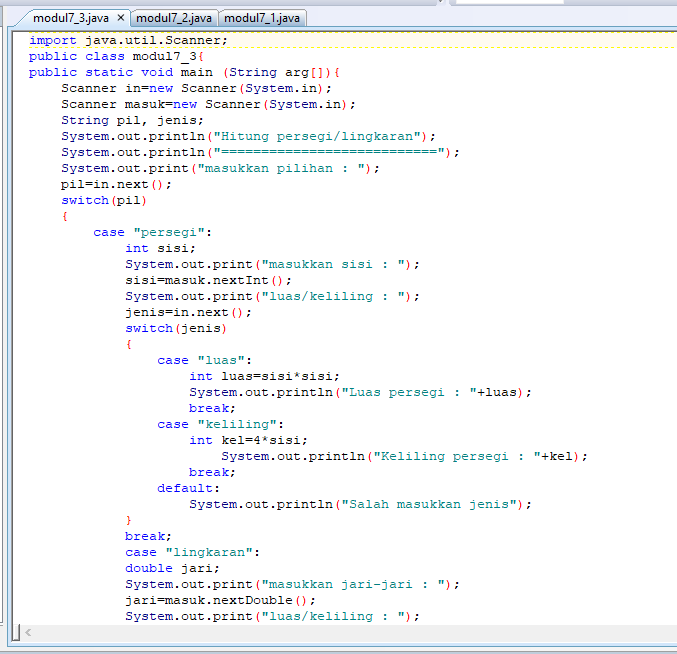
\includegraphics[width=\linewidth]{image--007}\\
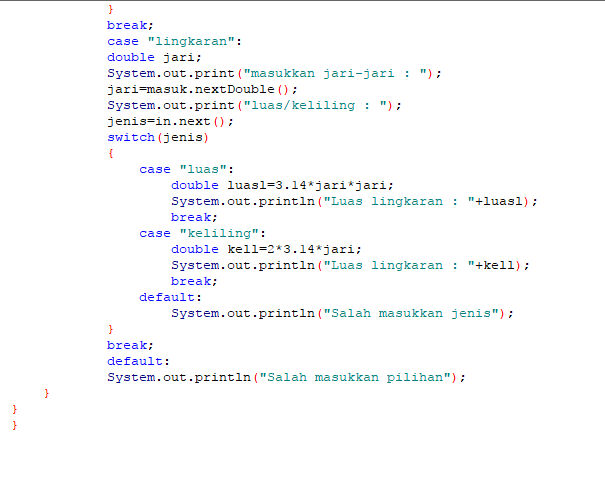
\includegraphics[width=\linewidth]{image--008}\\
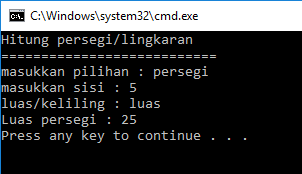
\includegraphics[scale=.6]{image--009}
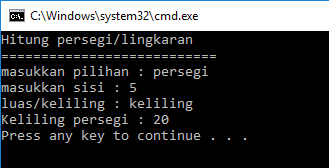
\includegraphics[scale=.6]{image--010}\\
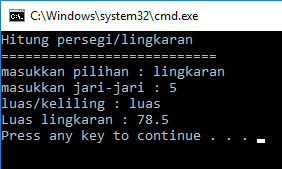
\includegraphics[scale=.6]{image--011}
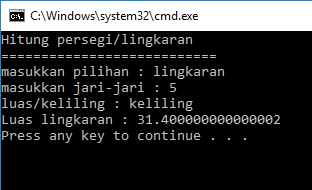
\includegraphics[scale=.6]{image--012}\\
Sebelum menhilangkan \texttt{break;} pada baris ke 32, program berjalan seperti yang diharapkan.

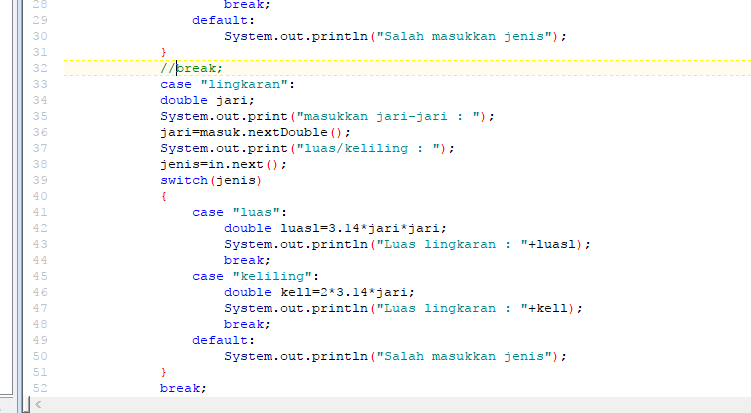
\includegraphics[width=\linewidth]{image--013}\\
Menghilangkan \texttt{break} pada baris ke 32\\
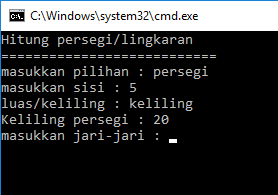
\includegraphics[scale=.6]{image--014}\\
Hasilnya saat program dijalankan, dan memasukkan pilihan persegi, setelah program selesai menghitung operasi dari persegi program akan melanjutkan ke case lingkaran, karena tidak adanya \texttt{break;} sebagai tanda berhenti dari \texttt{case}

\section{Latihan}
\paragraph{Masalah\\}
Buat program dengan if bertingkat untuk menampilkan harga mobil/motor
berdasarkan pilihan yang dimasukkan oleh user dengan ketentuan :
\begin{enumerate}[label=\alph*.]
	\item Pilih 1, jika pilihan mobil dan ada pilihan selanjutnya apakah Jazz (170 jt), Brio (120jt), Mobilio (170 jt)
	\item Pilih 2, jika pilihan motor dan ada pilihan selanjutnya Vario(16 jt), Beat (14 jt),Vixion(20 jt)
\end{enumerate}

\paragraph{Penyelesaian\\}
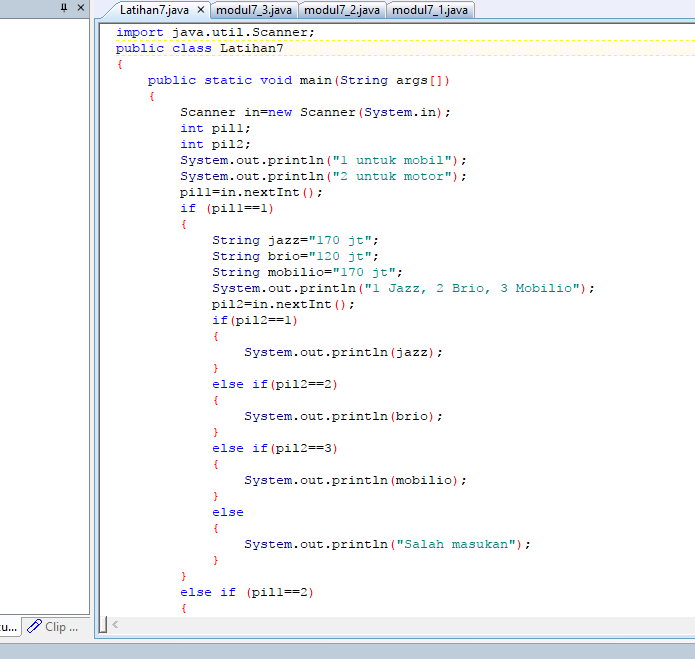
\includegraphics[width=\linewidth]{image--015}\\
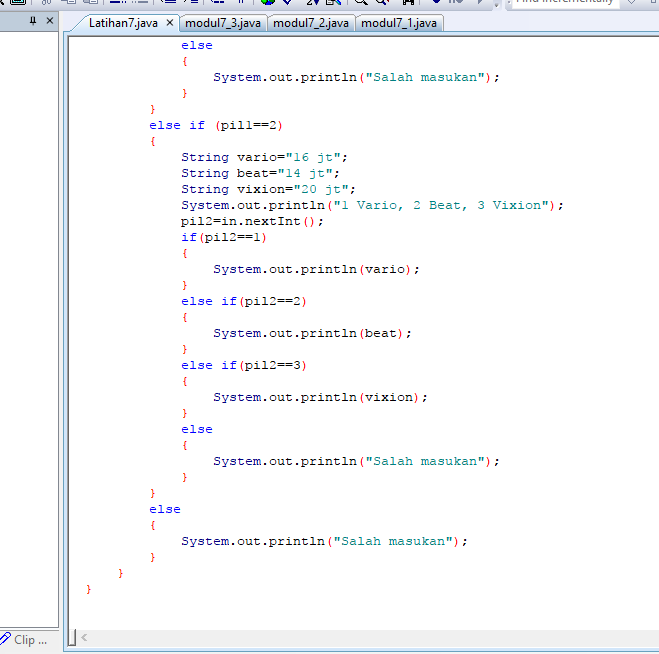
\includegraphics[width=\linewidth]{image--016}\\
{\bfseries Kode}
\begin{lstlisting}
import java.util.Scanner;
public class Latihan6
{
    public static void main(String args[])
    {
        Scanner in=new Scanner(System.in);
        int pil1;
        int pil2;
        System.out.println("1 untuk mobil");
        System.out.println("2 untuk motor");
        pil1=in.nextInt();
        if (pil1==1)
        {
            String jazz="170 jt";
            String brio="120 jt";
            String mobilio="170 jt";
            System.out.println("1 Jazz, 2 Brio, 3 Mobilio");
            pil2=in.nextInt();
            if(pil2==1)
            {
                System.out.println(jazz);
            }
            else if(pil2==2)
            {
                System.out.println(brio);
            }
            else if(pil2==3)
            {
                System.out.println(mobilio);
            }
            else
            {
                System.out.println("Salah masukan");
            }
        }
        else if (pil1==2)
        {
            String vario="16 jt";
            String beat="14 jt";
            String vixion="20 jt";
            System.out.println("1 Vario, 2 Beat, 3 Vixion");
            pil2=in.nextInt();
            if(pil2==1)
            {
                System.out.println(vario);
            }
            else if(pil2==2)
            {
                System.out.println(beat);
            }
            else if(pil2==3)
            {
                System.out.println(vixion);
            }
            else
            {
                System.out.println("Salah masukan");
            }
        }
        else
        {
            System.out.println("Salah masukan");
        }
    }
}
\end{lstlisting}
\paragraph{}
Pada program diatas kendaran dikategorikan menjadi dua, input 1 untuk kategori mobil, dan input 2 untuk mobil, jika input selain 1 dan 2 program akan menjalankan \texttt{System.out.println("Salah masukan");}
\paragraph{}
Didalam seleksi \texttt{if} dengan kondisi pil1==1 dan pil1==2 terdapat seleksi \texttt{if}lagi, yang memiliki kondisi 1 - 3 yang jika salah satu terpenuhi, program menjalankan \texttt{System.out.println("}\textit{variabel}\texttt{");} yang mana variabel berisi harga dari mobil atau motor yang sudah dideklarasikan. Jika variabel pil2 bukan 1 - 3, program akan menjalankan System.out.println("Salah masukan");

\section{Tugas}
\paragraph{Masalah\\}
Buat program dengan switch bertingkat untuk menampilkan besaran SPA yang harus
dibayar untuk kuliah di STMIK AKAKOM berdasarkan jenjang dan jurusan yang dipilih
dengan ketentuan :
\begin{table}[!ht]
	\begin{tabular}{|l|l|l|}
		\hline
		\multicolumn{1}{|c|}{\textbf{TK,KA,MI (D3)}} & \multicolumn{1}{c|}{\textbf{TI(S1)}} & \multicolumn{1}{c|}{\textbf{SI(S1)}} \\ \hline
		10.000.000                                   & 13.000.000                           & 12.000.000                           \\ \hline
	\end{tabular}
\end{table}
\paragraph{Penyelesaian\\}
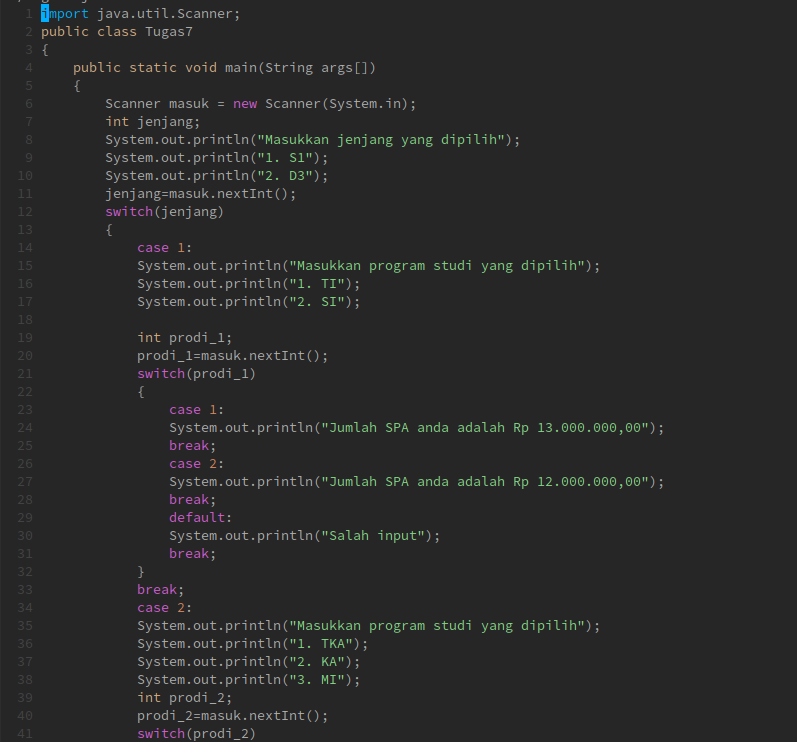
\includegraphics[width=\linewidth]{tugas-1}\\
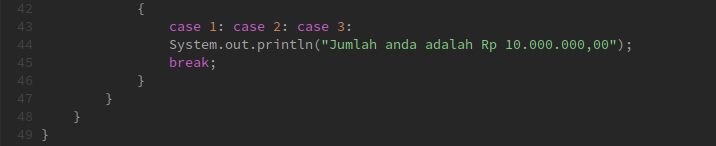
\includegraphics[width=\linewidth]{tugas-2}\\
{\bfseries Kode}
\begin{lstlisting}
import java.util.Scanner;
public class Tugas7
{
    public static void main(String args[])
    {
        Scanner masuk = new Scanner(System.in);
        int jenjang;
        System.out.println("Masukkan jenjang yang dipilih");
        System.out.println("1. S1");
        System.out.println("2. D3");
        jenjang=masuk.nextInt();
        switch(jenjang)
        {
            case 1:
    	    System.out.println("Masukkan program studi yang dipilih");
            System.out.println("1. TI");
            System.out.println("2. SI");
            
    	    int prodi_1;
            prodi_1=masuk.nextInt();
            switch(prodi_1)
            {
                case 1:
                System.out.println("Jumlah SPA anda adalah Rp 13.000.000,00");
                break;
                case 2:
                System.out.println("Jumlah SPA anda adalah Rp 12.000.000,00");
                break;
                default:
                System.out.println("Salah input");
                break;
            }
            break;
            case 2:
            System.out.println("Masukkan program studi yang dipilih");
            System.out.println("1. TKA");              
            System.out.println("2. KA");
            System.out.println("3. MI");
    	    int prodi_2;
            prodi_2=masuk.nextInt();
            switch(prodi_2)
            {
                case 1: case 2: case 3:
                System.out.println("Jumlah anda adalah Rp 10.000.000,00");
                break;
            }
        }
    }
}
\end{lstlisting}
\paragraph{Penjelasan\\}
Pada program untuk menampilkan besaran SPA diatas saya membagi jurusan menjadi dua, yaitu S1 dan D3, case 1 untuk S1, dan case 2  untuk D3. Untuk case 1, terdiri dari dua case dan satu default, case 1 menampilkan SPA untuk program studi TI, sedangkan case2 menampilkan SPA untuk program studi SI.
\paragraph{}
Sedangkan untuk case 2, terdiri dari 3 case, namun semuanya akan menjalankan fungsi yang sama, yaitu \texttt{System.out.println("Jumlah anda adalah Rp 10.000.000,00");}

\newpage
{\bfseries Output\\}
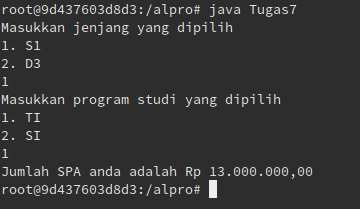
\includegraphics[scale=.6]{tugas-3}
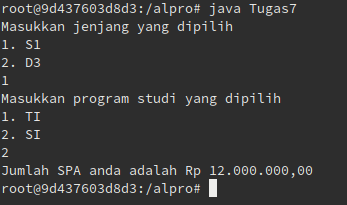
\includegraphics[scale=.6]{tugas-4}
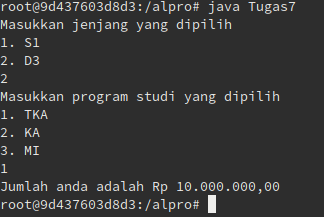
\includegraphics[scale=.6]{tugas-5}
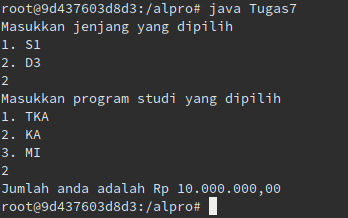
\includegraphics[scale=.6]{tugas-6}
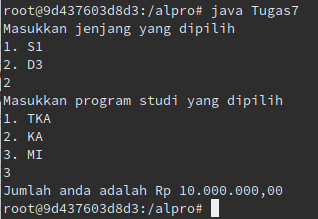
\includegraphics[scale=.6]{tugas-7}

\newpage
\section{Kesimpulan}
Mahasiswa dapat mengimplementasikan konsep seleksi bertingkat untuk menyelesaikan kasus

\end{document}